\documentclass[10pt,a4paper]{article}

\usepackage[utf8]{inputenc}
\usepackage[T1]{fontenc}	
\usepackage[italian]{babel}
\usepackage{amsmath}
\usepackage{amsfonts}
\usepackage{amssymb}
\usepackage{graphicx}

\usepackage[left=2cm,right=2cm,top=2cm,bottom=2cm]{geometry}
\geometry{a4paper}

\usepackage{booktabs} % for much better looking tables
\usepackage{verbatim}
\usepackage{subfig} % make it possible to include more than one captioned figure/table in a single 

% pacchetti che mi fanno schifo ma uso lo stesso (Bob è scemo, ma anche Ale...)
\usepackage[cdot, thickqspace, squaren]{SIunits}
% il miglior pacchetto che potessi desiderare
\usepackage{float}
% macro che mi piacciono
\def\code#1{\texttt{#1}}


\title{Misura del rapporto $e/m$}
\author{Gruppo BL \\ Candido Alessandro, Luzio Andrea, Mazziotti Fabrizio}

\begin{document}

\maketitle

\section{Elettroni in campo magnetico}
Dopo aver inserito il bulbo di vetro nel suo socket e acceso i vari alimentatori, si ha che gli atomi di $He$ all'interno dell'ampolla emettono radiazione nel visibile in seguito agli urti con gli elettroni. Questo consente di visualizzare il pennello elettronico e misurarne l'orbita (vedi \figurename{~\ref{fig:ex1}}).

\begin{figure}[H]
	\centering
	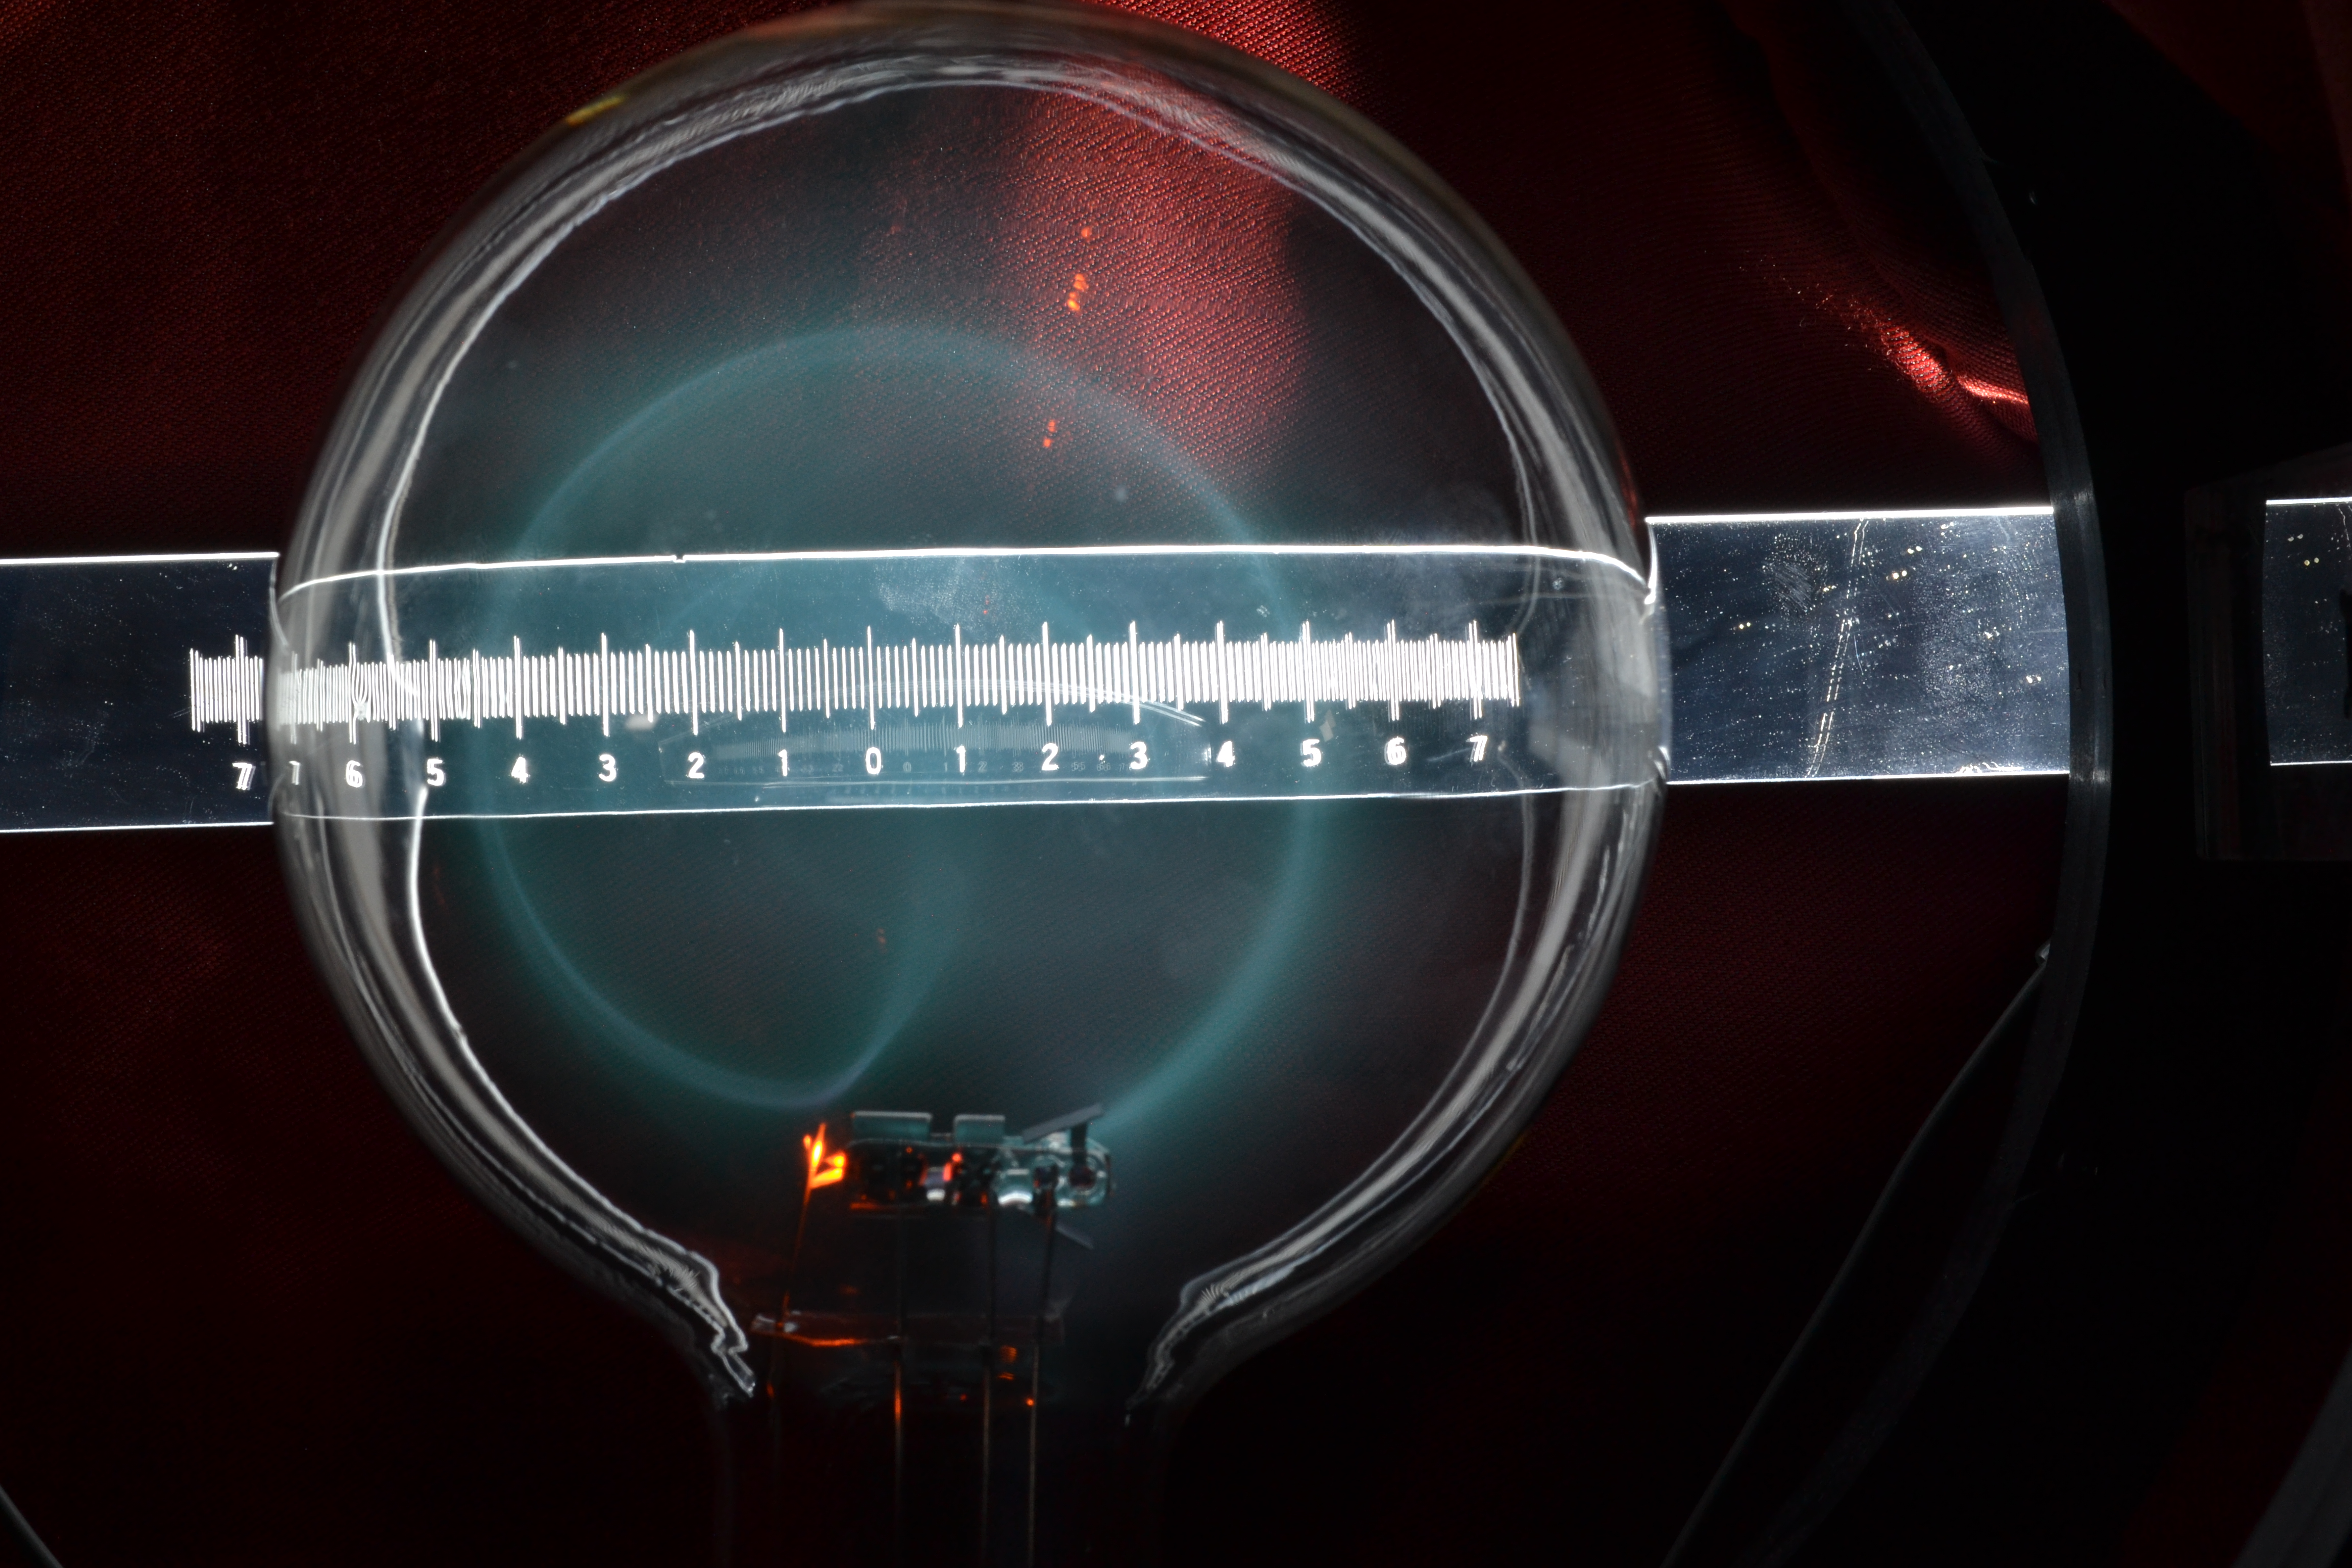
\includegraphics[width=0.8\textwidth]{../MisuraEM/2017-02-24/DSC_0025.jpg}
	\caption{Immagine esemplificativa del fenomeno osservato}
	\label{fig:ex1}
\end{figure}

\subsection{Emissione per effetto termoionico}

Si è fissato i valori di $I_{Coil} = \unit{1.17}{A}$ e $V_{Acc} = \unit{230}{V}$ e si è variata la tensione $V_{Heat}$ responsabile dell'emissione degli elettroni per vedere se il raggio della traiettoria dipende da essa.
Per tensioni $V_{Heat}$ di $\unit{6-5}{V}$ non si osserva nessuna variazione dell'orbita degli elettroni. Quando invece $V_{Heat} = \unit{4-3}{V}$ si osserva che la traccia si divide e va a formare un'elica..
%e giustificare perché il raggio è crescente con V_Heat

\subsection{Condizioni ottimali per le fotografie}

Ci si è posti nelle condizioni che si ritenevano ottimali (messo il panno scuro, fissata la posizione della macchina fotografica e il suo ingrandimento, per una successiva unica correzione delle immagini, illuminato la scala graduata) per scattare le foto con la macchina digitale e si è fissato $V_{Heat} = \unit{6}{V}$. 


\subsection{Acquisizione fotografie e prime stime di $e/m$}

In primo luogo si è mantenuta fissa $I_{Coil} = \unit{1.30 \pm 0.01}{A}$ e si è variata la tensione di accelerazione per misurare il raggio di curvatura dell'orbita circolare (r). Durante la fase di presa dati si sono stimati i vari raggi con la scala graduata per verificare l'ordine di grandezza di e/m, utilizzando le formule \eqref{eq:em} e \eqref{eq:vacc}. 

\begin{equation}
	\frac{e}{m} = \frac{v_e}{B_z r}
	\label{eq:em}
\end{equation}

\begin{equation}
\frac{1}{2} m v_e^2 = e V_{acc}
\label{eq:vacc}
\end{equation}

Si è ottenuto  $e/m \approx \unit{1.5-1.6~10^{11}}{C/Kg}$, in ottimo accordo con il valore atteso ($e/m_{th} = \unit{1.75~10^{11}}{C/Kg}$).

% forse dovrei fare un paragrafo in cui ammetto che come errori abbiamo preso un digit, tipo: \paragraph{Osservazione} Si è considerato ...
% sono d'accordo a scrivere quali errori abbiamo considerato ma secondo me non in un paragrafo a parte ma all'interno della sezione inerente, altrimenti è tutto troppo frammentato
\subsection{Risultati dei fit}

Per ottenere una misurata più accurata del raggio dell'orbita, e quindi di $e/m$ in ultima analisi, si è proceduto come segue:
\begin{itemize}
	\item si sono digitalizzate le fotografie;
	\item per ciascuna immagine è stato eseguito un best-fit a una circonferenza;
	\item sempre tramite fit si è trovato il fattore di calibrazione $pixel/cm$;
	\item si sono corretti i raggi ottenuti considerando l'effetto prospettico.
\end{itemize}

\paragraph{Digitalizzazione immagini} Per digitalizzare le immagini si è impiegato il software \emph{GetData Graph Digitizer} (uno di quelli suggeriti) andando a selezionare alcuni punti in corrispondenza dell'orbita luminosa (vedi \figurename{~\ref{fig:ex1}}.
I punti sono presi a coppie: le 4 coordinate così risultanti sono state poi utilizzate per stimare gli errori sui punti stessi, oltre ovviamente ai valor medi; operativamente per ogni "punto efficace" sono stati digitalizzati un punto sul margine interno della fascia luminosa e uno sul margine esterno.\footnote{I punti non sono stati presi su le zone estremali della fascia luminosa, come a stimare un errore massimo, ma piuttosto cercando di emulare una semilarghezza a metà altezza, considerando una successiva trattazione statistica.}

Oltre ai punti sull'orbita sono stati digitalizzati anche dei punti sul righello luminoso, in particolare sono stati presi i seguenti accorgimenti:
\begin{enumerate}
	\item si sono digitalizzati un punto ogni $\unit{5}{\milli\meter}$, cioè uno ogni 5 tacchette;
	\item per ovviare alle differenze fra le tacche indicanti multipli interi e semiinteri del cm si sono considerate le tacche traslate di $\unit{1}{\milli\meter}$ rispetto a tali valori (i.e.: $\unit{11}{\milli\meter}$, $\unit{16}{\milli\meter}$, $\unit{21}{\milli\meter}$, \dots);
	\item si è scelto di digitalizzare per ogni tacca l'estremità inferiore;
	\item si sono digitalizzati 11 punti, corrispondenti a tacche del righello abbastanza centrate rispetto al bulbo.
\end{enumerate}

Per quel che riguarda il terzo punto si è scelto di operare in questo modo così da evitare un errore aggiuntivo dovuto a una cattiva definizione dei punti da digitalizzare: nella foto in esame un punto come il centro della tacca è indistinguibile da quelli che stanno appena sopra o appena sotto di lui, mentre l'estremo inferiore è chiaramente distinguibile.

Il punto 4 invece è stato necessario per evitare di incorrere in un eccessiva deformazine del righello a causa della distorsione ottica dovuta al bulbo di vetro.

\paragraph{Fit circolari} Per ottenere i raggi delle circonferenza descritti dall'orbita degli elettroni si sono eseguiti dei fit analitici di circonferenze sui punti digitalizzati. Il metodo di fit seguito corrisponde a quello descritto in \emph{I.Kàsa, "A Circle Fitting Procedure and Its Error Analysis"}.
Si sono calcolati anche i rispettivi $\chi^2$, considerando come residuo quadratico il quadrato della distanza di ogni punto digitalizzato dalla circonferenza di fit normalizzato con la somma dei quadrati degli errori sulle coordinate $x$ e $y$.
Si riportano a titolo di esempio alcuni valori ottenuti in \tablename{~\ref{tab:rpchi2}}

\begin{figure}[H]
	\centering
	\resizebox{0.3\textwidth}{!}{
		\input{../tabelle/tab_somer.txt}}
	\captionof{table}{Alcuni raggi ottenuti dai fit con relativi errori percentuali e $\chi^2$}
	\label{tab:rpchi2}
\end{figure}

Si riporta anche l'immagine del risultato di un fit circolare in \figurename{~\ref{fig:fitcfr}}. Si fa notare che è evidenziato anche il centro della circonferenza di fit, mentre per quanto riguarda gli errori sui punti digitalizzati sono pressoché invisibili nella foto (fatta eccezione per pochi), e quello che viene visualizzato sono le estremità delle barre di errore (che si è scelto appositamente di non ridurre in modo da segnalare la presenza dei punti, e consentire, nei pochi casi in cui è possibile, di apprezzare l'errore, che sarebbe stato coperto da qualsiasi altro marcatore).

\begin{figure}[H]
	\centering
	\includegraphics[width=0.8\textwidth]{../grafici/39.pdf}
	\caption{Risultato di un fit (linea continua) e punti digitalizzati (croci)}
	\label{fig:fitcfr}
\end{figure}

\paragraph{Calibrazione delle immagini} Ottenuti i raggi in $pixel$ si è dunque cercato il fattore di conversione per passare a unità fisiche (cm). Per fare ciò si sono sfruttati i valori digitalizzati dei punti corrispondenti alle tacche del righello luminoso.

Si specifica innanzi tutto che gli errori sulle coordinate di tali punti sono stati stimati considerando la larghezza di tacca nella direzione orizzontale del righello e la sfrangiatura del fine tacca nela direzione verticale.\footnote{Anche in questo caso, come nella nota precedente, l'errore è inteso in senso quanto più possibile statistico, e non come errore massimo.}
In questo caso l'errore è stato assunto costante per tutti i punti, dato che le tacche di un righello presentano poca variabilità (a meno di significativo deteriorarmento, caso che non si è presentato).

Si è dunque eseguito un primo fit per determinare l'asse del righello, fittando le coordinate $x$ e $y$ dei punti con una retta affine.
Si sono poi proiettati i punti sulla retta trovata in modo analitico\footnote{Semplici calcoli di geometria analitica danno la formula della proiezione di un punto su una retta.}, e secondo tale formula si è propagato l'errore su tali proiezioni.

Si sono dunque calcolate le distanze di queste proiezioni dalla prima di esse (considerata come la più a sinistra nelle foto).


\section{Valutazione errori sistematici}

\subsection{Errore dovuto alla geometria proiettiva}
Il piano della scala graduata è diverso dal piano dell'orbita, quindi si deve tener conto di ciò. Si è misurata la distanza della lente della fotocamera dal piano del righello illuminato presente nelle foto($D$), e anche la distanza dal piano dell'orbita degli elettroni sempre rispetto alla lente($d$).
Si riportano in \tablename(\ref{}).

$D = 52.5 \pm 0.2$
$d = 45.0 \pm 0.4$

Il fattore dovuto alla prospettiva risulta pari a $\unit{0.86 \pm 0.01}{}$. 
%da finire e riportare tabella con i valori nuovi ottenuti per r e i relativi valori di e/m

\paragraph{Osservazione}
Un ulteriore verifica che bisogna fare è che il piano contenente l'orbita sia parallelo a quello contenente la lente della fotocamera, altrimenti le immagini prese non risultano essere circonferenze ma ellissi. A tal proposito si sono effettuati fit analitici ellittici per quantificare eventuali discrepanze dovute al non parallelismo tra i due piani, ottenendo una correzione ai raggi delle orbite di un'ulteriore $0,5\%$.
% percentuale stimata grossolanamente tra quasi tutte le foto, ma direi trascurabile quindi l'osservazione finisce qui.

\subsection{Effetto di distorsione dovuto alla rifrazione del bulbo}
%Si consiglia di prendere una foto della scala graduata (illuminata) posta dietro la seconda bobina in assenza il bulbo di vetro, per valutare successivamente l’effetto di distorsione introdotto dalla rifrazione del bulbo.

\subsection{Variazione $B_z(r)$/$B_z^{MAX}$}
%punto 3.d della scheda sarebbe?

Per meglio stimare la componente $B_z$ presente sulla traiettoria del fascio elettronico si è fatta una scansione con la sonda a effetto Hall facendola scorrere nella guida. Si sono ottenuti i dati in figura.\\

%\begin{figure}[h!]
%	\centering
%	\includegraphics[width=0.80\textwidth]{../figure/B_di_r.png}
%	\caption{Dati sperimentali scansione in $r$ di $B_z$ e relativo fit. Sulle ordinate si è rappresentato direttamente il valore di tensione output della sonda effetto Hall, misurato con il multimetro.Sovrapposto vi è un fit della curva teorica}
%	\label{task6.3}
%\end{figure}

Si è dunque tentato un fit con una curva teorica. Essa è stata stimata numericamente poiché gli autori non conoscono formule analitiche per gli integrali coinvolti (integrazione della formula di Biot-Savart nella circonferenza). Sono stati lasciati come parametri di fit il raggio delle bobine ($R$), la distanza bobina centro ($z$), la corrente circolante moltiplicata pesata con il numero di spire e la costante paramagnetica del vuoto ($I$), un offset rispetto al punto $r=0$ ($a$). Si sono ottenuti i seguenti risultati:\\

0.0043+/-0.0019

0.16916+/-0.00018

0.184+/-0.012

0.189+/-0.01

 
 

\section{Calcolo di e/m}

%Trovare la media dei valori ottenuti per e/m con l’errore statistico

%Riportare in un grafico (Bz r)^2 in funzione di Vacc


\end{document}